% --------------------------------------------------
% DOCUMENT CLASS
% --------------------------------------------------

\documentclass[
presentation.tex
]{subfiles}

\begin{document}

\section{Model}
	
% --------------------------------------------------
% SLIDE
% --------------------------------------------------
	
	\begin{frame}{Agents}

	The model has four agents:
	\begin{itemize}
	
	\item the representative household maximizes utility;
	
	\item firms producing intermediate goods minimize costs and maximize profit flow;
	
	\item firms producing final goods maximize profit.

	\item the monetary authority determines the interest rate, aiming to control inflation and pursuing economic growth.
	
	\end{itemize}		

	\end{frame}

% --------------------------------------------------
% SLIDE
% --------------------------------------------------

	\begin{frame}{Model Structure}
		
		\begin{figure}[h!]
		\centering
		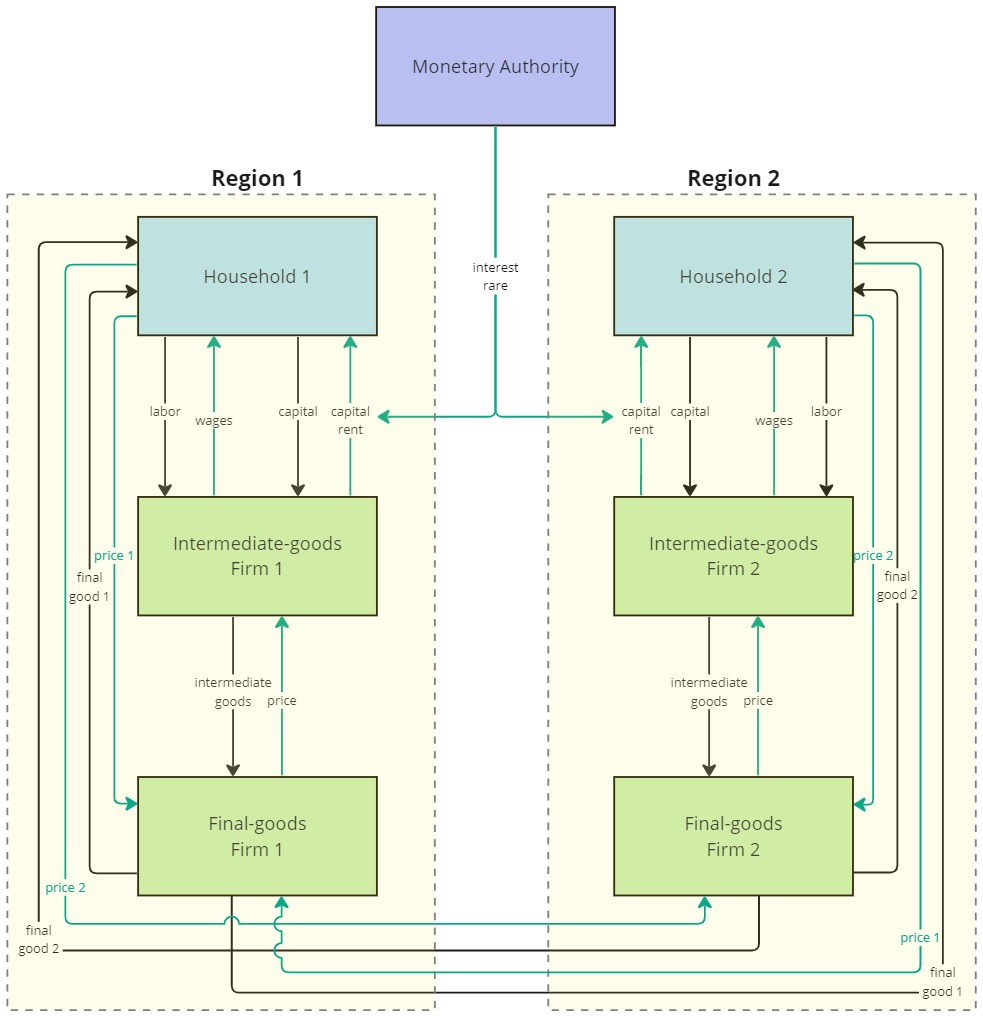
\includegraphics[width=\textwidth]{flowchart}
		\caption{Model Diagram}
		\label{fig:model-diagram}
		\end{figure}	
		
	\end{frame}

% --------------------------------------------------
% SLIDE
% --------------------------------------------------

\begin{frame}{Household Maximization Problem}
	
	\begin{align}
		\label{eq:household-utility-function}
		\max_{C_t,L_t,K_{t+1}}: \quad & U(C_t,L_t) = \E \sum_{t=0}^{\infty} \beta^t \left(\frac{C_t^{1-\sigma}}{1-\sigma} - \phi \frac{L_t^{1+\varphi}}{1+\varphi} \right) \\
		\label{eq:household-budget-constraint}
		\st: \quad & P_t (C_t + I_t) = W_t L_t + R_t K_t + \Pi_t \\
		\label{eq:law-of-motion-for-capital}
		\quad & K_{t+1} = (1-\delta)K_t + I_t \\
		\quad & C_t,L_t,K_{t+1} \geq 0 \text{ ; $K_0$ given.} \nonumber
	\end{align}
	
\end{frame}

% --------------------------------------------------
% SLIDE
% --------------------------------------------------

	\begin{frame}{Final-goods Firm Maximization Problem}
	
	\begin{align}
		\label{eq:final-good-firm-max-problem}
		\max_{Y_{jt}}: &\quad \Pi_t = P_t Y_t - \int_{0}^{1} P_{jt} Y_{jt} \dif j\\
		\label{eq:final-good-firm-bundle-rule}
		\st: & \quad Y_t = \left( \int_{0}^{1} Y_{jt}^{\frac{\psi-1}{\psi}} \dif j \right)^{\frac{\psi}{\psi-1}}
	\end{align}
	
	
	\end{frame}

% --------------------------------------------------
% SLIDE
% --------------------------------------------------

	\begin{frame}{Intermediate-goods Firm Problems}
		
	Cost Minimization Problem:	
	
	\begin{align}
		\label{eq:int-good-firm-total-cost}
		\min_{K_{jt}, L_{jt}}: \quad & R_t K_{jt} + W_t L_{jt} \\
		\label{eq:int-good-firm-production-function}
		\st: \quad & Y_{jt} = Z_{At} K_{jt}^\alpha L_{jt}^{1-\alpha}
	\end{align}	
				
	\end{frame}

% --------------------------------------------------
% SLIDE
% --------------------------------------------------

\begin{frame}{Intermediate-goods Firm Problems}
	
	Price Stickiness and Profit Flow, Calvo's Rule \cite{calvo_staggered_1983}:
	
	\begin{align}
		& \quad \mathbb{P}(P_t=P_{t-1})=\theta \\
		\max_{P_{jt}}: & \quad \E \sum_{s=0}^{\infty} \left\{ \frac{ \theta^s \left[ P_{jt} Y_{j,t+s} - TC_{j,t+s} \right] }{\prod_{k=0}^{s-1}(1+R_{t+k})} \right\} \label{eq:int-good-firm-optimal-price-problem} \\
		\st: & \quad Y_{jt} = Y_t \left( \frac{P_t}{P_{jt}} \right)^{\psi} %\tag{\ref{eq:final-good-firm-FOC}}
	\end{align}	
	
\end{frame}

% --------------------------------------------------
% SLIDE
% --------------------------------------------------

\begin{frame}{Monetary Authority}
	
	Taylor's Rule \cite{taylor_discretion_1993}
	
	\begin{align}
		\label{eq:monetary-policy}
		\frac{R_t}{R} =
		\left( \frac{R_{t-1}}{R} \right)^{\gamma_R}  \left[
		\left( \frac{\pi_t}{\pi} \right)^{\gamma_\pi}
		\left( \frac{Y_t}{Y} \right)^{\gamma_Y} \right]^{1-\gamma_R} Z_{Mt}
	\end{align}	
	
	
\end{frame}

% --------------------------------------------------
% SLIDE
% --------------------------------------------------

\begin{frame}{Stochastic Shocks}
	
	Productivity Shock:
	\begin{align}
		\ln{Z_{At}} = (1-\rho_A)\ln{Z_A} + \rho_A\ln{Z_{A,t-1}} + \varepsilon_{At} \label{eq:productivity-shock}
	\end{align}
	
	Monetary Policy Shock:
	\begin{align}
		\ln{Z_{Mt}} = (1-\rho_M)\ln{Z_{M}} + \rho_M\ln{Z_{M,t-1}} + \varepsilon_{Mt} \label{eq:monetary-shock}
	\end{align}
	
	
\end{frame}

% --------------------------------------------------
% SLIDE
% --------------------------------------------------

\begin{frame}[allowframebreaks]{Model Structure}
	
	{\singlespacing

Square system of 16 variables and 16 equations:

\begin{itemize}
	\item from the household problem: $C_t, L_t, K_{t+1}$;
	\item from the final-good firm problem: $Y_{jt}, P_t$;
	\item from the intermediate-good firm problems: $K_{jt}, L_{jt}, P_t^\ast$;
	\item from the market clearing condition: $Y_t, I_t$;
	\item prices: $W_t, R_t, \Lambda_t, \pi_t$;
	\item shocks: $Z_{At}, Z_{Mt}$.
\end{itemize}

	} % \singlespacing

\end{frame}

% --------------------------------------------------
% SLIDE
% --------------------------------------------------

\begin{frame}[allowframebreaks]{Model Structure}

	{\singlespacing

Equations:

\begin{enumerate}
	\item Labor Supply:
	\begin{align}
		\frac{\phi L_t^{\varphi}}{C_t^{-\sigma}} = \frac{W_t}{P_t}
		%\tag{\ref{eq:household-labor-supply}}
	\end{align}
	
	\item Household Euler Equation:
	\begin{align}
		\left( \frac{\mathbb{E}_t C_{t+1}}{C_t} \right)^\sigma = \beta \left[ (1-\delta) + \mathbb{E}_t \left(\frac{R_{t+1}}{P_{t+1}}\right) \right]
		%\tag{\ref{eq:household-euler-equation}}
	\end{align}
	
	\item Budget Constraint: 
	\begin{align}
		P_t (C_t + I_t) = W_t L_t + R_t K_t + \Pi_t
		%\tag{\ref{eq:household-budget-constraint}}
	\end{align}
	
	\item Law of Motion for Capital:
	\begin{align}
		K_{t+1} = (1-\delta)K_t + I_t
		%\tag{\ref{eq:law-of-motion-for-capital}}
	\end{align}
	
	\item Bundle Technology:
	\begin{align}
		Y_t = \left( \int_{0}^{1} Y_{jt}^{\frac{\psi-1}{\psi}} \dif j \right)^{\frac{\psi}{\psi-1}}
		%\tag{\ref{eq:final-good-firm-bundle-rule}}
	\end{align}
	
	\item General Price Level:
	\begin{align}
		P_t = \left[ \theta P_{t-1}^{1-\psi} + (1-\theta) P_t^{\ast 1-\psi} \right]^\frac{1}{1-\psi}
		%\tag{\ref{eq:general-price-level}}
	\end{align}
	
	\item Capital Demand:
	\begin{align}
		K_{jt} = \alpha Y_{jt} \frac{\Lambda_t}{R_t}
		%\tag{\ref{eq:int-good-firm-FOC-Kt}}
	\end{align}
	
	\item Labor Demand:
	\begin{align}
		L_{jt} = (1-\alpha) Y_{jt} \frac{\Lambda_t}{W_t}
		%\tag{\ref{eq:int-good-firm-FOC-Lt}}
	\end{align}
	
	% \item Marginal Rate of Substitution of Factors (\ref{eq:int-good-firm-TMRS}):
	% \[ \frac{K_{jt}}{L_{jt}} = \left( \frac{\alpha}{1-\alpha} \right) \frac{W_t}{R_t} \]
	
	\item Marginal Cost:
	\begin{align}
		\Lambda_t = \frac{1}{Z_{At}} \left( \frac{R_t}{\alpha} \right)^{\alpha} \left( \frac{W_t}{1-\alpha} \right)^{1-\alpha}
		%\tag{\ref{eq:int-good-firm-MC-2}}
	\end{align}
	
	\item Production Function:
	\begin{align}
		Y_{jt} = Z_{At} K_{jt}^\alpha L_{jt}^{1-\alpha}
		%\tag{\ref{eq:int-good-firm-production-function}}
	\end{align}
	
	\item Optimal Price:
	\begin{align}
		P_t^\ast = \frac{\psi}{\psi-1} \cdot \frac{ \E \sum_{s=0}^{\infty} \left\{ \theta^s Y_{j,t+s} \Lambda_{t+s} / \prod_{k=0}^{s-1}(1+R_{t+k}) \right\} } {\E \sum_{s=0}^{\infty} \left\{ \theta^s Y_{j,t+s} / \prod_{k=0}^{s-1}(1 + R_{t+k}) \right\}} %\tag{\ref{eq:int-good-firm-optimal-price-FOC-3}}
	\end{align}
	
	\item Market Clearing Condition:
	\begin{align}
		Y_t = C_t + I_t
		%\tag{\ref{eq:market-clearing-condition}}
	\end{align}
	
	\item Monetary Policy:
	\begin{align}
		\frac{R_t}{R} = \left( 
		\frac{R_{t-1}}{R} \right)^{\gamma_R} \left[ \left(
		\frac{\pi_t}{\pi} \right)^{\gamma_\pi} \left( 
		\frac{Y_t}{Y} \right)^{\gamma_Y} \right]^{1-\gamma_R} Z_{Mt}
		%\tag{\ref{eq:monetary-policy}}
	\end{align}
	
	\item Gross Inflation Rate:
	\begin{align}
		\pi_t = \frac{P_t}{P_{t-1}}
		%\tag{\ref{eq:gross-inflation-rate}}
	\end{align}
	
	\item Productivity Shock:
	\begin{align}
		\ln{Z_{At}} = (1-\rho_A)\ln{Z_A} + \rho_A\ln{Z_{A,t-1}} + \varepsilon_{At}
		%\tag{\ref{eq:productivity-shock}}
	\end{align}
	
	\item Monetary Shock:
	\begin{align}
		\ln{Z_{Mt}} = (1-\rho_M)\ln{Z_{M}} + \rho_M\ln{Z_{M,t-1}} + \varepsilon_{Mt}
		%\tag{\ref{eq:monetary-shock}}
	\end{align}
	
\end{enumerate}		
		
	} % \singlespacing
	
\end{frame}

% --------------------------------------------------
% SLIDE
% --------------------------------------------------

\subsection{Steady State}

\begin{frame}{Steady State}
	
	\centering \huge Steady State
	
\end{frame}

% --------------------------------------------------
% SLIDE
% --------------------------------------------------

\subsection{Log-linearization}

\begin{frame}{}
	
	
	
	
\end{frame}

% --------------------------------------------------
% SLIDE
% --------------------------------------------------

\begin{frame}{}
	
	
	
	
\end{frame}

% --------------------------------------------------
% SLIDE
% --------------------------------------------------

\begin{frame}{Características}

Além disso, também teremos características específicas:

\begin{itemize}
	\item regra de \textcite{calvo_staggered_1983}: gerar fricções nominais nos preços dos bens, alterando as relações de equilíbrio do sistema, gerando a não-neutralidade da moeda no curto prazo, \textcite[p.191]{costa_junior_understanding_2016}.
	
	\item os choques estocásticos estarão presentes na produtividade das firmas e nas preferências da família representativa.
	
	\item regionalização do modelo: um índice para a região estudada e o restante do Brasil, de tal forma que teremos as famílias, a firma de bens finais e as firmas de bens intermediários de cada região.
	
	\item as famílias não terão mobilidade, mas os bens intermediários e finais terão, e esse será o elo para conectar as duas regiões.
\end{itemize}

\end{frame}	

\end{document}